
\providecommand{\sSet}{s\mathcal{S}et}%

\section{始元素与终元素}\label{sec:f-initial-and-terminal-elements}

本节中，我们完成\cref{dig:terminal-elements-quasi-category}中概述的论证，%
证明拟范畴中\trTerminal{}\trElement{}的综合定义与 Joyal \cite[4.1]{bib61}%
最先引入的解析定义相一致。我们证明\trTerminal{}\trElement{}的四个综合定义%
——(i) 最先出现于\cref{def:initial-terminal-element}中的那个；(ii) 即%
\cref{lem:minimal-data}的那个；(iii) 作为\cref{prop:terminal-initial-trivial-fibration}%
出现的那个；以及 (iv) 文献中常见的那个（见例如 \cite{bib88}）——与%
\trTerminal{}\trElement{}的两个解析定义 (v) 与 (vi) 之间的等价；Joyal 已证明%
后二者彼此等价 \cite[4.2]{bib61}。

\begin{proposition}\label{prop:terminal-element-equivalences}
对于\trQuasiCategory{} $A$ 与\trElement{} $t\colon 1\to A$，以下条件等价：
\begin{enumerate}[label=(\roman*)]
\item \trElement{} $t$ 定义了唯一\trFunctor
\begin{center}
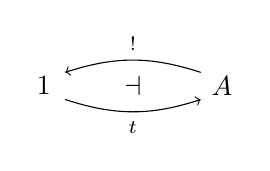
\begin{tikzpicture}[x=1.4em,y=1.4em]
  \node (One) at (0,0)   {$1$};
  \node (A)   at (4.6,0) {$A$};
  \draw[->] (4.05,0.35) to[bend right=18] node[above]{$\scriptstyle !$} (0.55,0.35);
  \node at (2.3,0) {$\dashv$};
  \draw[->] (0.55,-0.35) to[bend right=18] node[below]{$\scriptstyle t$} (4.05,-0.35);
\end{tikzpicture}
\end{center}
的\trRightAdjoint{}。
\item 存在一个\trNaturalTransformation
\begin{center}
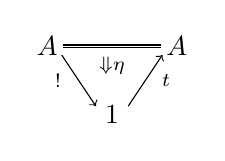
\begin{tikzpicture}[x=1.3em,y=1.3em]
  \node (L) at (0,0)    {$A$};
  \node (R) at (3.6,0)  {$A$};
  \draw[double] (0.45,0) -- (3.15,0);
  \node at (1.8,-0.55) {$\scriptstyle\Downarrow\eta$};
  \node (B) at (1.8,-1.9) {$1$};
  \draw[->] (0.4,-0.24) -- (1.35,-1.66);
  \node at (0.3,-0.95) {$\scriptstyle !$};
  \draw[->] (2.25,-1.66) -- (3.2,-0.24);
  \node at (3.3,-0.95) {$\scriptstyle t$};
\end{tikzpicture}
\end{center}
使得其分量 $\eta t$ 是一个\trIsomorphism{}。
\item 定义域投影\trFunctor
\begin{center}
$\mathrm{Hom}_{A}(A,t)\xrightarrow[\sim]{\ p_{0}\ }A$
\end{center}
定义一个\trTrivialFibration{}。
\item 对任何\trElement{} $a\colon 1\to A$，\trMappingSpace{}
$\mathrm{Hom}_{A}(a,t)$ 是\trContractible{}。
\item 投影\trFunctor
\begin{center}
$A_{/t}\xrightarrow{\ \sim\ }A$
\end{center}
——其定义域是 $A$ 在 $t$ 之上的切片——是一个\trTrivialFibration{}。
\item $A$ 中末顶点为 $t$ 的任何\trSphere{}都容许一个填充体：
\begin{center}
\begin{tikzpicture}[x=1.9em,y=1.4em]
  \node (o)  at (0,1.3)    {$1$};
  \node (pd) at (3.4,1.3)  {$\partial\Delta[n]$};
  \node (a)  at (7.4,1.3)  {$A$};
  \node (dn) at (3.4,-1.5) {$\Delta[n]$};
  \draw[->] (o) -- node[below]{$\scriptstyle\{n\}$} (pd);
  \draw[->] (pd) -- (a);
  \draw[->] (o) to[bend left=28] node[above,pos=0.5]{$\scriptstyle t$} (a);
  \draw[right hook->] (3.4,0.95) -- (3.4,-1.15);
  \draw[->,dashed] (3.75,-1.3) -- (7.0,1.0);
\end{tikzpicture}
\end{center}
\end{enumerate}
当这些条件成立时，$t$ 定义了 $A$ 的一个\textbf{\trTerminal{}\trElement}。
\end{proposition}

\begin{proof}
拆解 (i)：要定义\trAdjunction{} $!\dashv t$，所须的全部数据不过是一个%
\trUnit{}\trNaturalTransformation{} $\eta\colon\mathrm{id}_{A}\Rightarrow t!$，%
使得其分量 $\eta t=\mathrm{id}_{t}$ 为恒等。但正如\cref{lem:minimal-data}所%
证明的，若 $\eta t$ 可逆，则它必为恒等。这就证明了 (i) 与 (ii) 的等价性。

\cref{prop:terminal-initial-trivial-fibration}在任何\trInfinityCosmos{}中
建立了 (i) 与 (iii) 的等价性。由\cref{cor:discrete-cartesian-trivial-contractible}与%
\cref{cor:domain-projection-from-element}，定义域投影\trFunctor{}是一个%
\trTrivialFibration，当且仅当其诸\trFiber{} $\mathrm{Hom}_{A}(a,t)$ 是%
\trContractible{}，这就证明了 (iii) 与 (iv) 的等价性。

由\cref{cor:slice-cone-point}，对\trQuasiCategory{}中的任何顶点 $t$，在%
\cref{prop:join-slice-adjunction}之切片构造的典范投影与定义域投影%
\trIsofibration{}之间存在一个\trEquivalence
\begin{center}
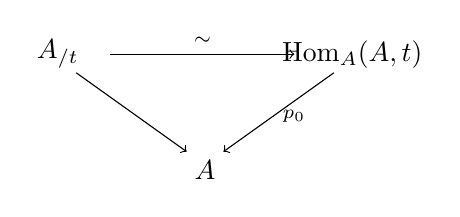
\begin{tikzpicture}[x=1.9em,y=1.5em]
  \node (at) at (0,1.3)    {$A_{/t}$};
  \node (h)  at (5.6,1.3)  {$\mathrm{Hom}_{A}(A,t)$};
  \node (a)  at (2.8,-1.5) {$A$};
  \draw[->] (1.0,1.3) -- node[above]{$\scriptstyle\sim$} (4.5,1.3);
  \draw[->] (0.35,0.85) -- (2.45,-1.05);
  \draw[->] (5.25,0.85) -- node[right,pos=0.55]{$\scriptstyle p_{0}$} (3.15,-1.05);
\end{tikzpicture}
\end{center}
于是，由\trTwoOfThreeProperty，二者之中一条\trIsofibration{}是一个%
\trEquivalence，当且仅当另一条亦然，这就证明了 (iii) 与 (v) 的等价性。

依\cref{def:trivial-fibration}，投影 $A_{/t}\twoheadrightarrow A$ 是一个%
\trTrivialFibration，当且仅当对一切 $n\ge 0$，如下右提升性质成立
\begin{center}
\begin{tikzpicture}[x=1.9em,y=1.5em]
  \node (pd) at (0,1.3)    {$\partial\Delta[n]$};
  \node (at) at (4.4,1.3)  {$A_{/t}$};
  \node (dn) at (0,-1.5)   {$\Delta[n]$};
  \node (a)  at (4.4,-1.5) {$A$};
  \draw[->] (1.0,1.3) -- node[above]{$\scriptstyle u$} (3.3,1.3);
  \draw[right hook->] (0,0.9) -- (0,-1.1);
  \draw[->] (1.0,-1.5) -- node[below]{$\scriptstyle v$} (3.3,-1.5);
  \draw[->] (4.4,0.9) -- (4.4,-1.1);
  \draw[->,dashed] (0.5,-1.25) -- (3.6,1.0);
  \node at (1.7,-0.1) {$\scriptstyle w$};
\end{tikzpicture}
\end{center}
经\trAdjunction
\begin{center}
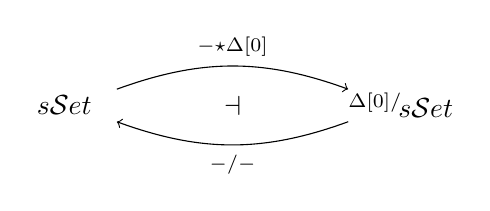
\begin{tikzpicture}[x=1.9em,y=1.4em]
  \node (s) at (0,0)   {$\sSet$};
  \node (j) at (6.4,0) {${}^{\Delta[0]/}\!\sSet$};
  \draw[->] (1.0,0.42) to[bend left=20] node[above]{$\scriptstyle-\star\Delta[0]$} (5.4,0.42);
  \node at (3.2,0) {$\dashv$};
  \draw[->] (5.4,-0.42) to[bend left=20] node[below]{$\scriptstyle-/-$} (1.0,-0.42);
\end{tikzpicture}
\end{center}
\trSphere{} $u\colon\partial\Delta[n]\to A_{/t}$ 经转置成为带末顶点 $t$ 的映射
$\Lambda^{n+1}[n+1]\to A$，而单纯形 $v\colon\Delta[n]\to A$ 则为该%
\trHorn{}的开口面提供一个填充体。于是，该\trLifting{}问题经转置便定义了
一个带末顶点 $t$ 的\trSphere{} $\partial\Delta[n+1]\to A$；所求的提升
$w\colon\Delta[n]\to A_{/t}$ 恰在这个经转置的\trSphere{}容许一个填充体时存在。
如此，我们便看到，右提升性质
\begin{center}
\begin{tikzpicture}[x=1.5em,y=1.5em]
  \node (fa) at (-2.4,0)  {$\forall n\ge 0$};
  \node (pd) at (0.4,1.3)  {$\partial\Delta[n]$};
  \node (at) at (4.8,1.3)  {$A_{/t}$};
  \node (dn) at (0.4,-1.5) {$\Delta[n]$};
  \node (a)  at (4.8,-1.5) {$A$};
  \draw[->] (1.4,1.3) -- node[above]{$\scriptstyle u$} (3.7,1.3);
  \draw[right hook->] (0.4,0.9) -- (0.4,-1.1);
  \draw[->] (1.4,-1.5) -- node[below]{$\scriptstyle v$} (3.7,-1.5);
  \draw[->] (4.8,0.9) -- (4.8,-1.1);
  \draw[->,dashed] (0.9,-1.25) -- (4.0,1.0);
  \node at (2.1,-0.1) {$\scriptstyle w$};
  \node at (7.4,0) {$\;\leftrightsquigarrow\;$};
  \begin{scope}[shift={(8.8,0)}]
  \node (o)   at (0,1.3)    {$1$};
  \node (pd2) at (3.4,1.3)  {$\partial\Delta[n]$};
  \node (a2)  at (7.4,1.3)  {$A$};
  \node (dn2) at (3.4,-1.5) {$\Delta[n]$};
  \draw[->] (o) -- node[below,pos=0.6]{$\scriptstyle\{n\}$} (pd2);
  \draw[->] (pd2) -- (a2);
  \draw[->] (o) to[bend left=25] node[above,pos=0.5]{$\scriptstyle t$} (a2);
  \draw[right hook->] (3.4,0.9) -- (3.4,-1.1);
  \draw[->,dashed] (3.75,-1.25) -- (7.0,1.0);
  \end{scope}
  \node (fa2) at (18.4,0) {$\forall n\ge 1$};
\end{tikzpicture}
\end{center}
互为转置，这就证明了 (v) 与 (vi) 的等价性。
\end{proof}

Joyal 的刻画 (vi) 有如下一个相对化的扩充：

\begin{lemma}\label{lem:relative-terminal-element-lifting}
设 $E$ 与 $B$ 是容有\trTerminal{}\trElement{}的\trQuasiCategory，且
$p\colon E\twoheadrightarrow B$ 是保持它们的\trIsofibration——意即：若 $t$
是 $E$ 的\trTerminal{}\trElement，则 $pt$ 是 $B$ 的\trTerminal{}\trElement{}。
那么任何如下形式的\trLifting{}问题都有解
\begin{center}
\begin{tikzpicture}[x=1.9em,y=1.4em]
  \node (o)  at (0,1.3)    {$1$};
  \node (pd) at (3.4,1.3)  {$\partial\Delta[n]$};
  \node (e)  at (7.6,1.3)  {$E$};
  \node (dn) at (3.4,-1.5) {$\Delta[n]$};
  \node (b)  at (7.6,-1.5) {$B$};
  \draw[->] (o) -- node[below]{$\scriptstyle\{n\}$} (pd);
  \draw[->] (pd) -- node[above]{$\scriptstyle u$} (e);
  \draw[->] (o) to[bend left=25] node[above,pos=0.5]{$\scriptstyle t$} (e);
  \draw[right hook->] (3.4,0.95) -- (3.4,-1.15);
  \draw[->,dashed] (3.75,-1.3) -- (7.2,1.0);
  \draw[->] (7.6,0.95) -- node[right]{$\scriptstyle p$} (7.6,-1.15);
  \draw[->] (dn) -- node[below]{$\scriptstyle v$} (b);
\end{tikzpicture}
\end{center}
\end{lemma}

\begin{proof}
利用 $E$ 中\trTerminal{}\trElement{} $t$ 的\trUniversalProperty{}以及%
\cref{prop:terminal-element-equivalences}(vi)，我们可以把\trSphere{} $u$ 扩充为
一个映射 $w\colon\Delta[n]\to E$。这就定义了两个映射
$pw\colon\Delta[n]\to B$ 与 $v\colon\Delta[n]\to B$，它们拥有公共边界
$pu\colon\partial\Delta[n]\to B$；由此可以定义一个\trSphere
$h\colon\partial\Delta[n+1]\to B$，使之满足 $h\delta^{n+1}=pw$ 与
$h\delta^{n}=v$——做法是：从退化\trSimplex{}
$pw\sigma^{n}\colon\Delta[n+1]\to B$ 出发，将其限制到边界上，再把该\trSphere{}中的
第 $n$ 个面替换为 $v\colon\Delta[n]\to B$。由构造，$h$ 把顶点 $\{n+1\}$ 送到 $pt$，而后者是
$B$ 的\trTerminal{}\trElement；于是我们便可以填充这个\trSphere，定义出一个单纯形
$k\colon\Delta[n+1]\to B$。

我们通过限制退化\trSimplex{} $w\sigma^{n}\colon\Delta[n+1]\to E$ 来构造
一个\trHorn{} $g\colon\Lambda^{n}[n+1]\to E$。这一对映射定义出陈述中那个
交换方块的因子分解：
\begin{center}
\begin{tikzpicture}[x=1.9em,y=1.5em]
  \node (pd) at (0,1.3)    {$\partial\Delta[n]$};
  \node (e)  at (3.2,1.3)  {$E$};
  \node (dn) at (0,-1.5)   {$\Delta[n]$};
  \node (b)  at (3.2,-1.5) {$B$};
  \draw[->] (1.0,1.3) -- node[above]{$\scriptstyle u$} (2.1,1.3);
  \draw[right hook->] (0,0.9) -- (0,-1.1);
  \draw[->] (1.0,-1.5) -- node[below]{$\scriptstyle v$} (2.1,-1.5);
  \draw[->] (3.2,0.9) -- node[right]{$\scriptstyle p$} (3.2,-1.1);
  \node at (4.7,0) {$=$};
  \begin{scope}[shift={(6.2,0)}]
  \node (pd2) at (0,1.3)    {$\partial\Delta[n]$};
  \node (la)  at (3.8,1.3)  {$\Lambda^{n}[n+1]$};
  \node (e2)  at (8.0,1.3)  {$E$};
  \node (dn2) at (0,-1.5)   {$\Delta[n]$};
  \node (dn1) at (3.8,-1.5) {$\Delta[n+1]$};
  \node (b2)  at (8.0,-1.5) {$B$};
  \draw[->] (1.0,1.3) -- node[above]{$\scriptstyle\delta^{n}$} (2.6,1.3);
  \draw[->] (5.1,1.3) -- node[above]{$\scriptstyle g$} (6.9,1.3);
  \draw[right hook->] (0,0.9) -- (0,-1.1);
  \draw[right hook->] (3.8,0.9) -- (3.8,-1.1);
  \draw[->,dashed] (4.15,-1.3) -- (7.6,1.0);
  \node at (6.15,-0.45) {$\scriptstyle\ell$};
  \draw[->] (8.0,0.9) -- node[right]{$\scriptstyle p$} (8.0,-1.1);
  \draw[->] (1.0,-1.5) -- node[below]{$\scriptstyle\delta^{n}$} (2.6,-1.5);
  \draw[->] (5.1,-1.5) -- node[below]{$\scriptstyle k$} (6.9,-1.5);
  \end{scope}
\end{tikzpicture}
\end{center}
由于这个交换矩形的中央竖直映射是一个内\trHorn{}包含，而其右手竖直映射是
拟范畴之间的一个\trIsofibration，故右边的\trLifting{}问题如所标记的那样有解
$\ell\colon\Delta[n+1]\to E$；于是显然，映射
$\ell\delta^{n}\colon\Delta[n]\to E$ 便为原来的\trLifting{}问题提供一个解。
\end{proof}

\subsection*{练习}

\begin{exercise}\label{ex:relative-lifting-arbitrary-functor}
证明：若 $A$ 与 $B$ 是容有\trTerminal{}\trElement{}的\trQuasiCategory，且
$f\colon A\to B$ 是一个保持诸\trTerminal{}\trElement{}的\trFunctor（未必是%
\trIsofibration），那么给定任何如下左图所示、其中 $t$ 是 $A$ 的%
\trTerminal{}\trElement{}的\trLifting{}问题
\begin{center}
\begin{tikzpicture}[x=1.9em,y=1.4em]
  \node (o)  at (0,1.3)    {$1$};
  \node (pd) at (3.4,1.3)  {$\partial\Delta[n]$};
  \node (a)  at (7.6,1.3)  {$A$};
  \node (dn) at (3.4,-1.5) {$\Delta[n]$};
  \node (b)  at (7.6,-1.5) {$B$};
  \draw[->] (o) -- node[below]{$\scriptstyle\{n\}$} (pd);
  \draw[->] (pd) -- (a);
  \draw[->] (o) to[bend left=25] node[above,pos=0.5]{$\scriptstyle t$} (a);
  \draw[right hook->] (3.4,0.95) -- (3.4,-1.15);
  \draw[->] (dn) -- (b);
  \draw[->] (7.6,0.95) -- node[right]{$\scriptstyle f$} (7.6,-1.15);
  \node at (9.8,0) {$\;\leftrightsquigarrow\;$};
  \begin{scope}[shift={(11.6,0)}]
  \node (pd2) at (0,1.3)    {$\partial\Delta[n]$};
  \node (a2)  at (4.4,1.3)  {$A$};
  \node (dn2) at (0,-1.5)   {$\Delta[n]$};
  \node (b2)  at (4.4,-1.5) {$B$};
  \draw[->] (1.0,1.3) -- (3.3,1.3);
  \draw[right hook->] (0,0.95) -- (0,-1.15);
  \draw[->] (1.0,-1.5) -- (3.3,-1.5);
  \draw[->] (4.4,0.95) -- node[right]{$\scriptstyle f$} (4.4,-1.15);
  \draw[->,dashed] (0.35,-1.3) -- (3.9,1.0);
  \node at (3.0,0.35) {$\scriptstyle\Downarrow\cong$};
  \end{scope}
\end{tikzpicture}
\end{center}
都存在如上右图所示的一个提升，使得左上三角在自然同构的意义下交换，而右下
三角严格交换。
\end{exercise}

\begin{exercise}\label{ex:initial-element-equivalences}
陈述并证明拟范畴中\trInitial{}\trElement{}的各种综合定义与解析定义之间的
等价。
\end{exercise}

